\documentclass[12pt]{article}
\usepackage[utf8]{inputenc}
\usepackage{gaml}
\usepackage{booktabs} % for better looking tables
\usepackage{multirow} % for multirow functionality

% refer to configurations.tex for the LaTeX setup of this template
\usepackage[english]{babel}

\title{\textbf{\textsf{Modeling and Simulation Project: Evacuation}}}
\date{\today}
\author{\textbf{Professor: Alexis Drogoul} \\ \\ Vu Trung Dung | dungvt2440071@usth.edu.vn }

% math
\usepackage{amsmath, amssymb}

% references
\usepackage[style=apa, backend=biber]{biblatex}
\addbibresource{bibliography.bib}

% fonts
\usepackage{helvet}
\usepackage{sectsty}
\allsectionsfont{\sffamily} % for section titltes use sans-serif
% \renewcommand{\familydefault}{\sfdefault} % comment out for sans-serif font
% \usepackage{sansmath} % comment out for sans-serif math font
% \sansmath % comment out for sans-serif math font

% margins
\usepackage{geometry}
\geometry{
  a4paper,
  total={170mm,257mm},
  left=25mm,
  right=25mm,
  top=30mm,
  bottom=30mm,
}

% no indentation when a new paragraph starts
\setlength{\parindent}{0cm}

% links
\usepackage{hyperref} % better links
\usepackage{color}    % nicer link colors
\definecolor{pigment}{rgb}{0.2, 0.2, 0.6}
\hypersetup{
  colorlinks = true, % Color links instead of ugly boxes
  urlcolor   = pigment, % Color for external hyperlinks
  linkcolor  = black, % Color for internal links
  citecolor  = pigment % Color for citations
}

% headers
\usepackage{fancyhdr}
\pagestyle{fancy}
\lhead{USTH - Modeling and Simulation Complex System- Prof. Alexis Drogoul}
\chead{}
\rhead{}

% example boxes
\usepackage{tcolorbox}
\newtcolorbox{examplebox}{
  colback=white,
  colframe=gray!30,
  title=Example,
  sharp corners,
  boxrule=0.5pt,
  coltitle=black
}

\newtcolorbox{codebox}{
  colback=white,
  colframe=gray!40,
  title=GAMA,
  sharp corners,
  boxrule=0.5pt,
  coltitle=black
}

% conditionals
\usepackage{ifthen}
\newboolean{showinstructions}
\newboolean{showexamples}
\newboolean{showexplanations}
\renewenvironment{examplebox}{%
  \ifthenelse{\boolean{showexamples}}%
    {\begin{tcolorbox}[colback=white, colframe=gray!30, title=Example, sharp corners, boxrule=0.5pt, coltitle=black]}%
    {\expandafter\comment}%
}{%
  \ifthenelse{\boolean{showexamples}}%
    {\end{tcolorbox}}%
    {\expandafter\endcomment}%
}

% Define a new environment for explanations
\newcommand{\explanation}[1]{%
  \ifthenelse{\boolean{showexplanations}}%
    {\textit{Explanation:} #1}%
    {\ignorespaces}%
}

% Define a new environment for instructions
\newcommand{\instructions}[1]{%
  \ifthenelse{\boolean{showinstructions}}%
    {#1}%
    {\ignorespaces}%
}

\makeatletter
\newcommand{\maketitlepage}{%
    % \begin{titlepage}
        \maketitle
        \thispagestyle{empty}
    % \end{titlepage}
}
\makeatother


% Optional user settings
\setboolean{showinstructions}{true} % set to false to hide instructions
\setboolean{showexamples}{true} % set to false to hide examples
\setboolean{showexplanations}{true} % set to false to hide explanations

\begin{document}
\maketitlepage

% --------------------------
% Abstract
% --------------------------
\begin{abstract}
\centering
Populations are increasingly vulnerable to disastrous natural or technological events, as demographic and urban growth lead to greater exposures of goods and people. Hanoi, for example, is particularly hard hit by flooding. Some districts on the banks of the Red River are also threatened by potential dike breaching. In the event of a levee failure, it is important to be able to evacuate the population living in these areas before the water arrives.
\end{abstract}




% --------------------------
% 1. Introduction
% --------------------------
\section{Introduction}


% --------------------------
% 1.1. Problem Statement
% --------------------------
\subsection{Problem Statement}
The goal of this project is to build an agent-based model of people evacuation, to have a better understanding of the evacuation process and to be able to test different evacuation strategies. The question to be answered is: \textbf{How to better manage the pedestrian evacuation of a population on a beach in a tsunami context?} \\

The goal is to optimize the evacuation process according to the following criteria:
\begin{itemize}
    \item Minimize the time people spend wandering on the roads to inform others about the threat.
    \item Maximize the number of people informed and evacuated.
    \item Minimize the total evacuation time as well.
\end{itemize}


% --------------------------
% 1.2. Problem Extensions
% --------------------------
\subsection{Project Extensions}
In this model, flooding will not be modeled by itself, just the behavior of residents in the face of the threat. People will only evacuate if they have been informed of the imminent risk of flooding. At the start of the simulation, we assume that all residents are located in their own homes and only 10\% of the population (randomly chosen) will be aware of this information. Once informed, people will evacuate to the shelter (the largest building in the area). A person observing someone evacuating (at a distance of less than 10m) will have a probability of 0.1 of evacuating in turn.

\begin{itemize}
\item[1] \textbf{Extension 1}: Only 10\% of the population go directly to the shelter when informed of the risk. The other will move to random buildings to inform other residents and search for the shelter.
\item[2] \textbf{Extensions 2}: Implement the multiple modalities of evacuation (car, motocycle, walking) and the possibility of blocking roads.
\item[3] \textbf{Extensions 3}: Experiment with different evacuation strategies of informing the threat to the 10\% of the population: those furthest from shelter, those closest to the shelter, or randomly selected.
\end{itemize}




% --------------------------
% 2. Implementation
% --------------------------
\section{Implementation}
In this section, I will describe the implementation of the agent-based model for the evacuation process. 

% --------------------------
% 2.1. Base Model
% --------------------------
\subsection{Base Model}
The base model include the following \textbf{species}:
\begin{itemize}
    \item \textbf{Inhabitant}: Represented as people that can move on the map, spread threat information, and evacuate to the shelter.
    \item \textbf{Buildings}: Represented as static objects where people can stay or move to for shelter.
    \item \textbf{Roads}: Represented as paths that people can use to move around the area.
    \item \textbf{Shelter}: Represented as the largest building in the area where people can evacuate to.
\end{itemize}

The people is randomly placed in their homes at initialization. To make it more realistic, I suppose that there are at maximum 5 people in each house. When the threat is announced, I randomly choose 10\% of the population to be informed. People who are informed have 10\% change to evacuate directly to the shelter, other will wander around to inform others and search for the shelter. In GAMA implementation, \textbf{inhabitant} species have included the skills \textbf{moving}, which allow them to move around through the roads. They realize the shelter if they found it at 20m distance. They stop moving when they reach the shelter and completely evacuate. \\

In my implementation, I suppose that \textbf{people don't revisit the same place they have been before}, so they will not wander around the same place, to increase the chance of finding the shelter. This is done by maintaining a list of visited places for each inhabitant. \\

The tsunami is not modeled in this base model, there is only the alert time before the tsunami arrives and the evacuation process. When tsunami strikes, it's often too late to inform and evacuate people. So the another way to express the question: \textbf{How effective are different evacuation processes in maximizing the number of evacuees within a limited time frame?} \\

According to that, the simulation start with the alert time, and the evacuation process will be stopped after a certain time or when all people have evacuated. \\

Note that to save the resources, I will destroy the inhabitant agents when they reach the shelter, after counting them as evacuated. \\

The most important part of the inhabitant behaviour is the \textbf{find\_shelter} reflex function, which is responsible for the evacuation process. The function is described as follows:

\begin{codebox}
\begin{lstlisting}[style=GAML]
reflex find_shelter when: target = nil and is_evacuating {
    if (shelter distance_to self < 1#m) {
        number_evacuted_people <- number_evacuted_people + 1;
        total_time_in_roads <- total_time_in_roads + (current_date - start_evacuating_date);
        total_evacuation_time <- total_evacuation_time + time;
        do die;
        return;
    }
    
    building target_building <- known_shelter ? shelter : nil;
    if (target_building = nil) {
        write("randomly find another shelter");
        if (shelter distance_to self < 20#m) {
            target_building <- shelter;
        }
        target_building <- one_of((building - visited_buildings) where each.is_safe);
    }
    visited_buildings << target_building;
    target <- any_location_in(target_building);
}
\end{lstlisting}
\end{codebox}

In this code, the \textbf{is\_evacuating} and \textbf{known\_shelter} are the agent's attributes that indicate the evacuation status and the knowledge of the shelter location. The \textbf{visited\_buildings} is the list of buildings that the agent has visited, to avoid revisiting the same place. The \textbf{number\_evacuted\_people} is the global variable that counts the number of people evacuated. The \textbf{total\_time\_in\_roads} and \textbf{total\_evacuation\_time} are the global variables that count the total time people spend wandering on the roads and the total evacuation time. Finally, the built-in attribute \textbf{target} to set to any location in the \textbf{target\_building} to move to that location. \\


% --------------------------
% 2.2. Extension 1
% --------------------------
\subsection{Extension 1}

As describe in the previous code, each inhabitant include the \textbf{known\_shelter} attribute to indicate if they know the shelter location. This is randomly set to 10\% of the population at the beginning of the simulation.


% --------------------------
% 2.3. Extension 2
% --------------------------
\subsection{Extension 2}

In this extension, I simulate the road heavily congested by cars and motorcycles, which block the way for pedestrians. Each inhabitant has their own mobilities which set randomly at the beginning of the simulation. The mobilities include \textbf{car}, \textbf{motorcycle}, and \textbf{walking}. \\

Here is the code represented the \textbf{road\_weights} of the roads in the simulation:
\begin{codebox}
\begin{lstlisting}[style=GAML]
global {
    reflex update_speed {
        road_weights <- road as_map (each::each.shape.perimeter / each.speed_rate);
    }
}

species road {
    float capacity <- 1 + shape.perimeter/10;
    float total_traffic_weight <- 0.0 
        update: sum((inhabitant at_distance 1) collect each.traffic_weight);
    float speed_rate <- 1.0 update:  exp(-total_traffic_weight/capacity) min: 0.1;
}
\end{lstlisting}
\end{codebox}

% --------------------------
% 2.4. Extension 3
% --------------------------
\subsection{Extension 3}

In this extension, I experiment with different evacuation strategies of informing the threat to the 10\% of the population: 
\begin{itemize}
    \item \textbf{Furthest}: Inform the threat to the 10\% of the population who are furthest from the shelter.
    \item \textbf{Closest}: Inform the threat to the 10\% of the population who are closest to the shelter.
    \item \textbf{Random}: Inform the threat to the 10\% of the population who are randomly selected.
\end{itemize}

In GAMA, I simply define the different strategies by setting the \textbf{known\_shelter} attribute of the different selected inhabitant agents. The code is as follows:

\begin{codebox}
\begin{lstlisting}[style=GAML]
if (initial_inform_strategy = "random") {
    write("Strategy: Random");
    ask nb_informing_people among inhabitant {
        do evacuate();
    }
} else if (initial_inform_strategy = "furthest") {
    write("Strategy: Furthest");
    ask nb_informing_people first (inhabitant sort_by -distance_to(shelter, each)) {
        do evacuate();
    }
} else {
    write("Strategy: Closest");
    ask nb_informing_people first (inhabitant sort_by distance_to(shelter, each)) {
        do evacuate();
    }
}
\end{lstlisting}
\end{codebox}

The experiment of different strategies I conducted will be presented in the next section.

% --------------------------
% 3. Experiments
% --------------------------
\section{Experiments}

\subsection{Pre-Definitions}

To have better presentation of the simulation, I define different colors for the different evacuate status of the inhabitant agents, which are:
\begin{itemize}
    \item \textbf{Evacuating/Informed}: Blue
    \item \textbf{Uninformed}: Yellow
\end{itemize}

And the different shape for the different mobilities of the inhabitant agents, which are:
\begin{itemize}
    \item \textbf{Car}: Square.
    \item \textbf{Motorcycle}: Triangle.
    \item \textbf{Walking}: Circle.
\end{itemize}

All of theses are showed in the Fig \ref{fig:mobilities}.

\begin{figure}
    \centering
    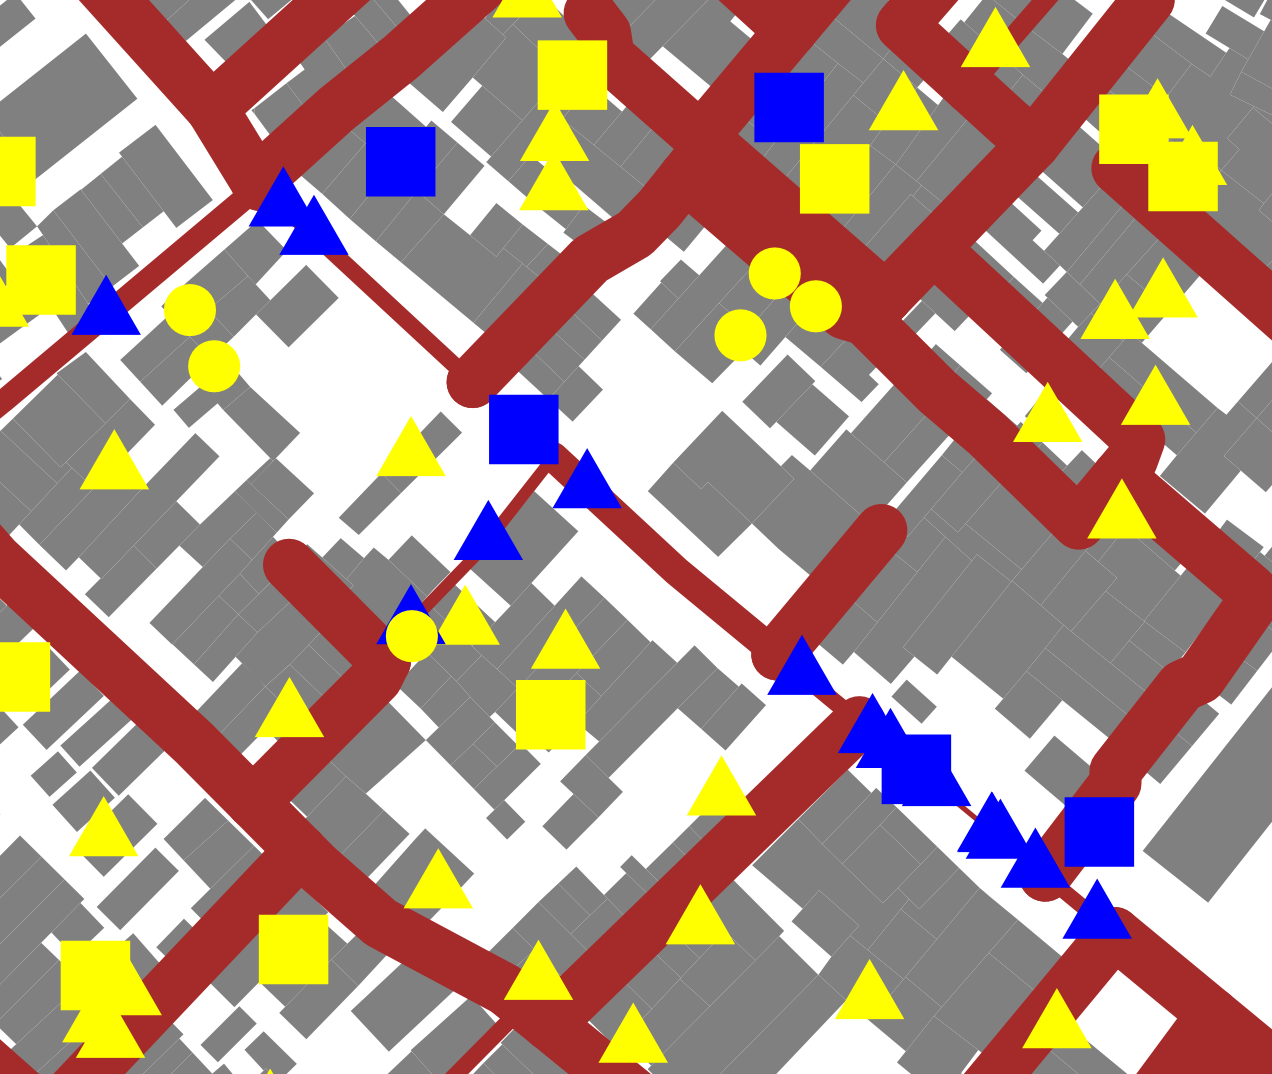
\includegraphics[width=0.6\textwidth]{../images/mobilities.png}
    \caption{Different mobilities of the inhabitant agents: Car (Square), Motorcycle (Triangle), Walking (Circle). Colors represent the evacuate status: Blue (Evacuating/Informed), Yellow (Uninformed).}
    \label{fig:mobilities}
\end{figure}

\subsection{Parameters}

The parameters of the simulation are set as follows (Fig \ref{fig:parameters}):
\begin{itemize}
    \item \textbf{Inform Strategy}: one of \{random, furthest, closest\}
    \item \textbf{Number of People}: default 1000
    \item \textbf{Alert Time}: the time before the tsunami arrives, default 120 minutes.
\end{itemize}

\begin{figure}
    \centering
    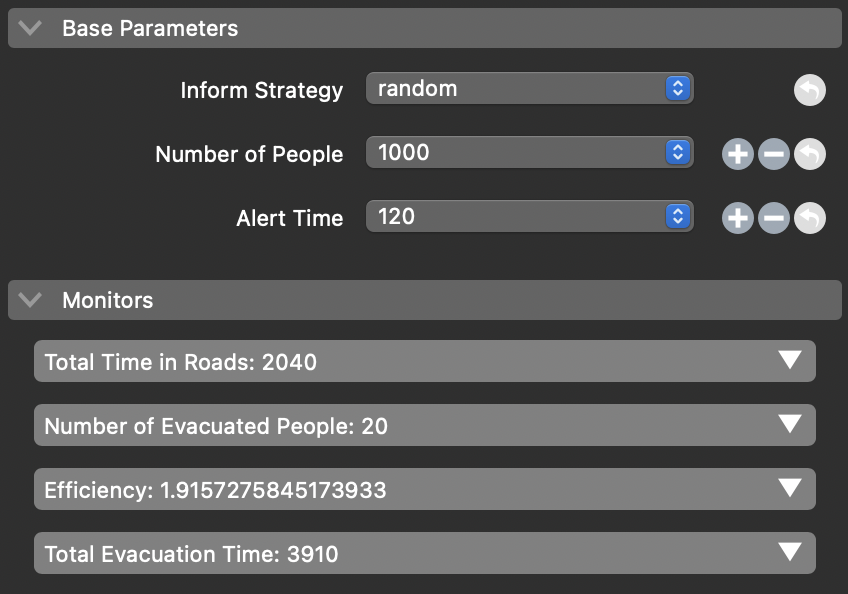
\includegraphics[width=0.6\textwidth]{../images/parameters.png}
    \caption{Parameters and Metrics of the simulation.}
    \label{fig:parameters}
\end{figure}

\subsection{Metrics}

To monitor and evaluate the evacuation process, I define the following metrics:
\begin{itemize}
    \item \textbf{Number of Evacuated People}: The number of people who have evacuated to the shelter before the tsunami arrives.
    \item \textbf{Total Time in Roads}: The total time people spend wandering on the roads to inform others and search for the shelter. To be specified, the time is counted from the time the inhabitant is informed and start evacuating until they reach the shelter.
    \item \textbf{Total Evacuation Time}: The time from the alert time until the last inhabitant evacuates to the shelter.
    \item \textbf{Efficiency}: The efficiency of the strategy.
\end{itemize}

The \textbf{Total Time in Roads} can be calculated by the formula:
\begin{align*}
    \text{Total Time in Roads} = \sum_{i=1}^{N} \text{T\_roads}_i
\end{align*}
\begin{align*}
    \text{T\_roads}_i = 
    \begin{cases}
        \text{t\_evacuated}_i - \text{t\_informed}_i & \text{if the inhabitant reaches the shelter} \\
        \text{t\_current} - \text{t\_informed}_i & \text{if the inhabitant is still on the road}
    \end{cases}
\end{align*}
where $\text{t\_evacuated}_i$ is the time the inhabitant $i$ reaches the shelter and $\text{t\_informed}_i$ is the time the inhabitant $i$ is informed and start evacuating, and N is the total of informed people. \\

The topic suggests the \textbf{Efficiency} of the strategy, which can be calculated by the formula:
\begin{align*}
    \text{Efficiency} = \frac{\text{Total Evacuation Time}}{\text{Total Time in Roads}}
\end{align*}

But after conducting the simulation, I found that this is not a good metric to evaluate the strategy. In the worst case, when the simulation stops because of running out of time, the total evacuation time equals the total simulation runtime, the total time spent on the roads could still be low if only 10\% of people were informed initially and went directly to the shelter without informing others. This scenario would yield a highest efficiency number despite being the worst strategy.\\

To correct this, I suggest the \textbf{Efficiency} metric to be calculated by the formula:
\begin{align*}
    \text{Efficiency} = \frac{\text{Total Evacuated people} \times \text{Alert Time}}{\text{Total Time in Roads} + 1}
\end{align*}

This metric will give a better evaluation of the strategy, as it tries to minimize the time people spend wandering on the roads to inform others and search for the shelter, and maximize the number of people informed, resulting in the total number of people evacuated. The $\text{+1}$ is added to avoid the division by zero. The scaling of the $\text{Alert Time}$ is added to make the division to be in the same unit.\\

Note that the chance of people successfully finding the shelter is random, and can't be controlled by the strategy. \textbf{The strategy only affects the number of people informed and the time they spend wandering on the roads, which possibility increases the chance of successfully evacuated people}.\\

\subsection{Results}

In this experiments, I conducted the simulation with different strategies and alert times. I also made the comparison between the different strategies by running them in parallel. About the map, I used the map of \textbf{Hanoi and the Red River} in the previous exercises. The shelter in this map is the one in the right-bottom corner (colored in green in the Fig \ref{fig:map}).\\ 

However, this building is too far from the others, which makes the evacuation process more difficult, since it's hard to people to realize it at distance 20m while wandering around. I made a change by selecting the building in the center-bottom of the map as the shelter. It is presented in red color in the Fig \ref{fig:map}. A quick experiment showed that in the settings of 3000 people and 2 hours of alert time, the number of evacuated people is increased to 298 compared to 248 of the previous shelter. Since the new shelter is more accessible, the results of comparison between the strategies are more reliable, as they eliminate the luck factor involved in finding the shelter and focus on the efficiency of the strategies.\\

\begin{figure}
    \centering
    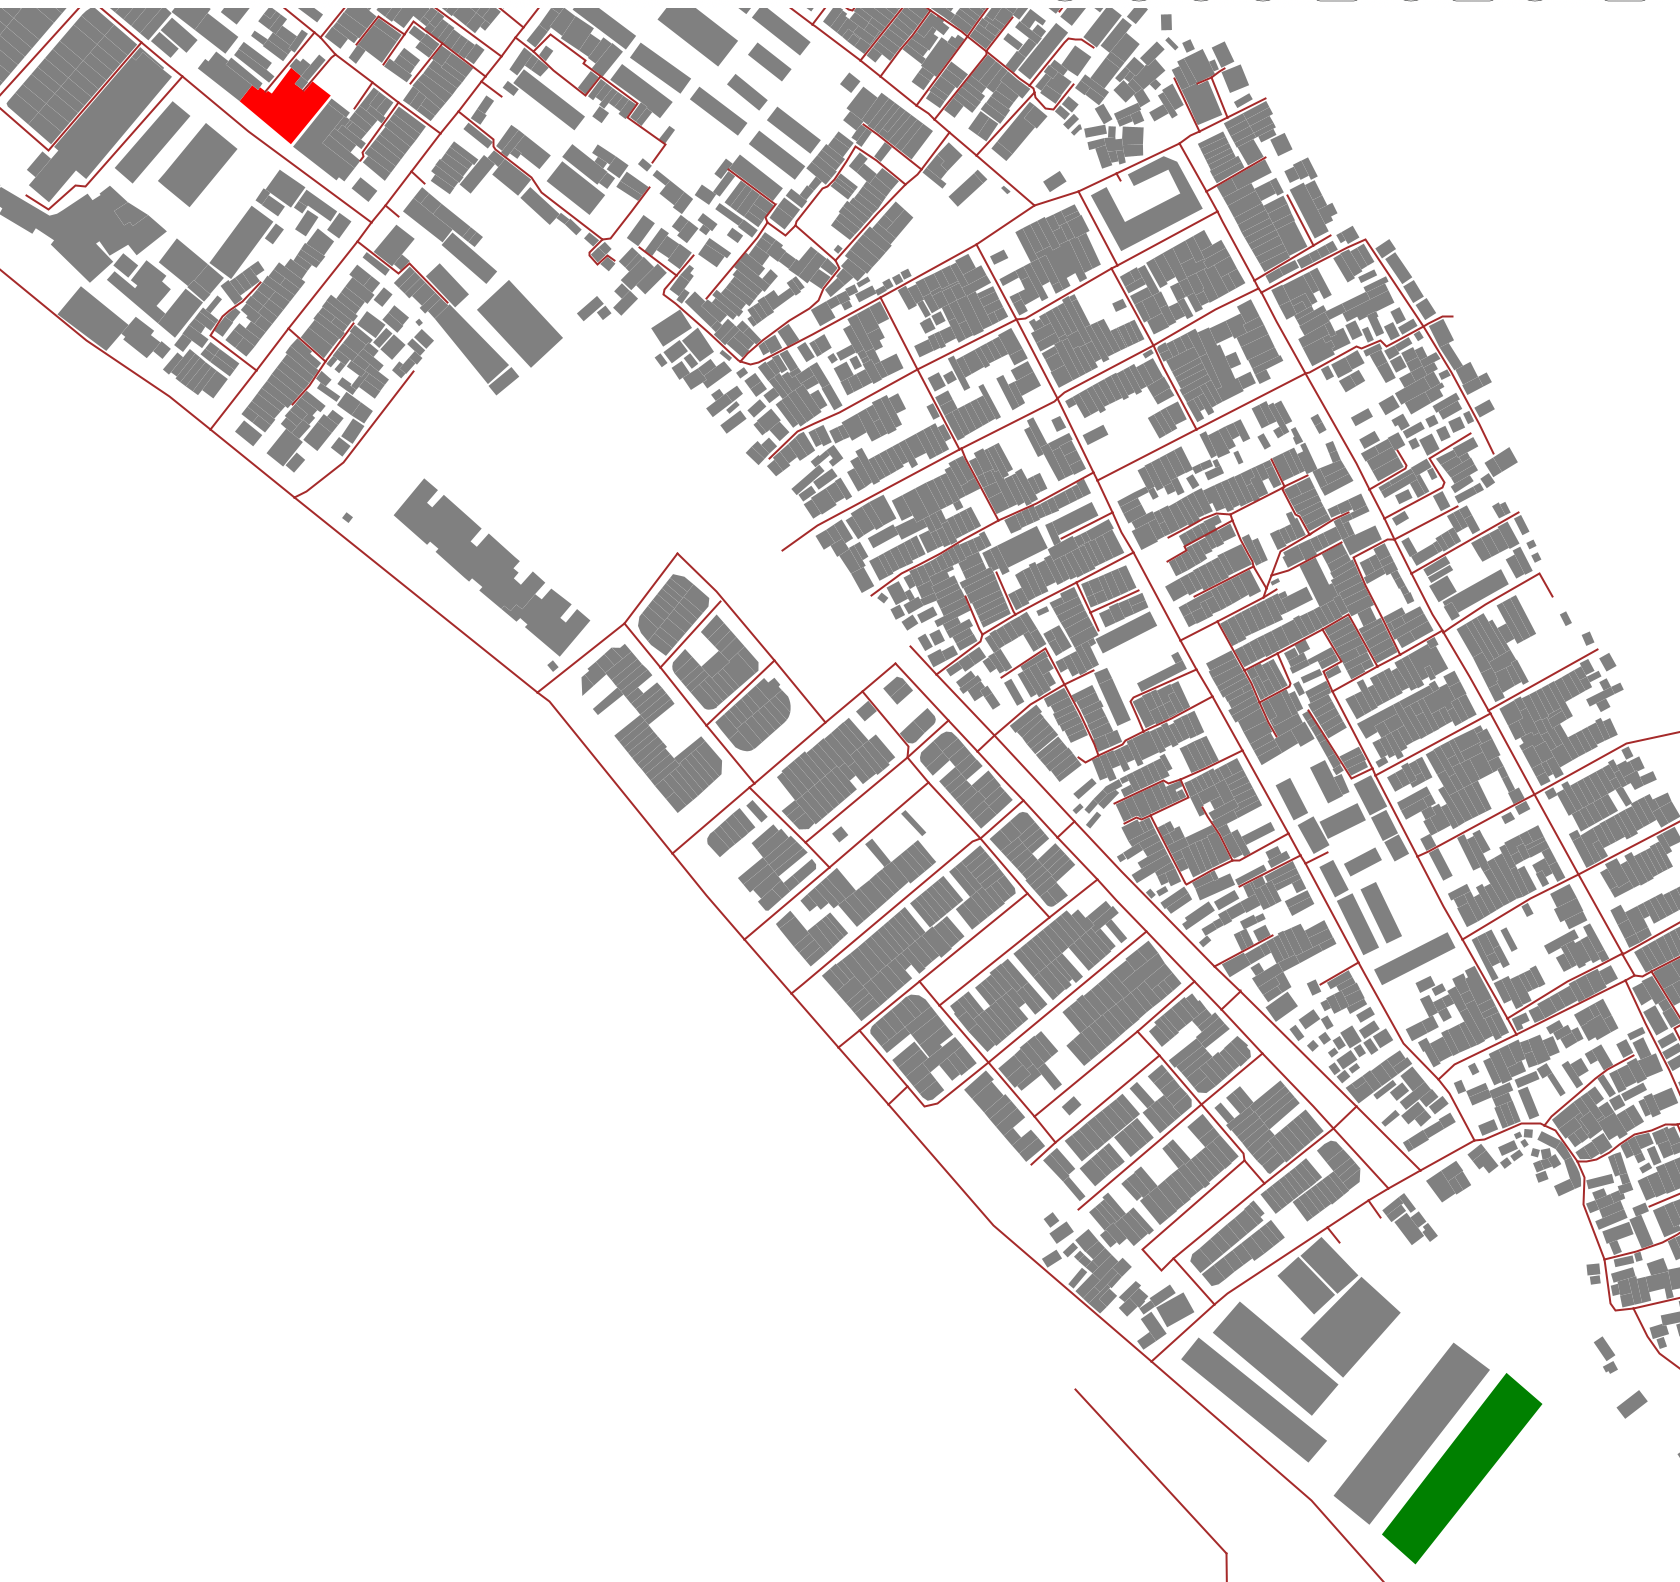
\includegraphics[width=0.6\textwidth]{../images/map0.png}
    \caption{The GIS data of Hanoi and the Red River. The largest building is in the bottom-right corner (colored in green). The shelter is in the center of the map (colored in red).}
    \label{fig:map}
\end{figure}

A single simulation of the evacuation process is presented in the Fig \ref{fig:results-single}. \\

The comparison of the different strategies in number of evacuated people is presented in the Fig \ref{fig:evacuees_over_time}. The experiment is conducted with 2000 and 4000 people, 20 minutes alert time among the different strategies. The results show that, at the settings of large number of people, the \textbf{closest} strategy is the one that save the most people, followed by the \textbf{furthest} strategy, and the \textbf{random} strategy is the least efficient. At smaller number of people, the three strategies have similar results. In all cases, the \textbf{random} strategy introduces the fastest evacuation process at the beginning. These findings can be explained by some reasons:
\begin{itemize}
    \item The \textbf{random} strategy is the fastest at the beginning because the people are randomly selected, which means they are distributed evenly across the map, so the people can start finding the shelter from diverse locations, which reduces the traffic congestion and the time people spend wandering on the roads, but the chance of people finding the shelter isn't increased.
    \item The \textbf{closest} strategy introduces the largest number of people saved because the people closest to the shelter have chance to inform others closed to the shelter as well, which increases the chance of people finding the shelter.
\end{itemize}

\begin{figure}
    \centering
    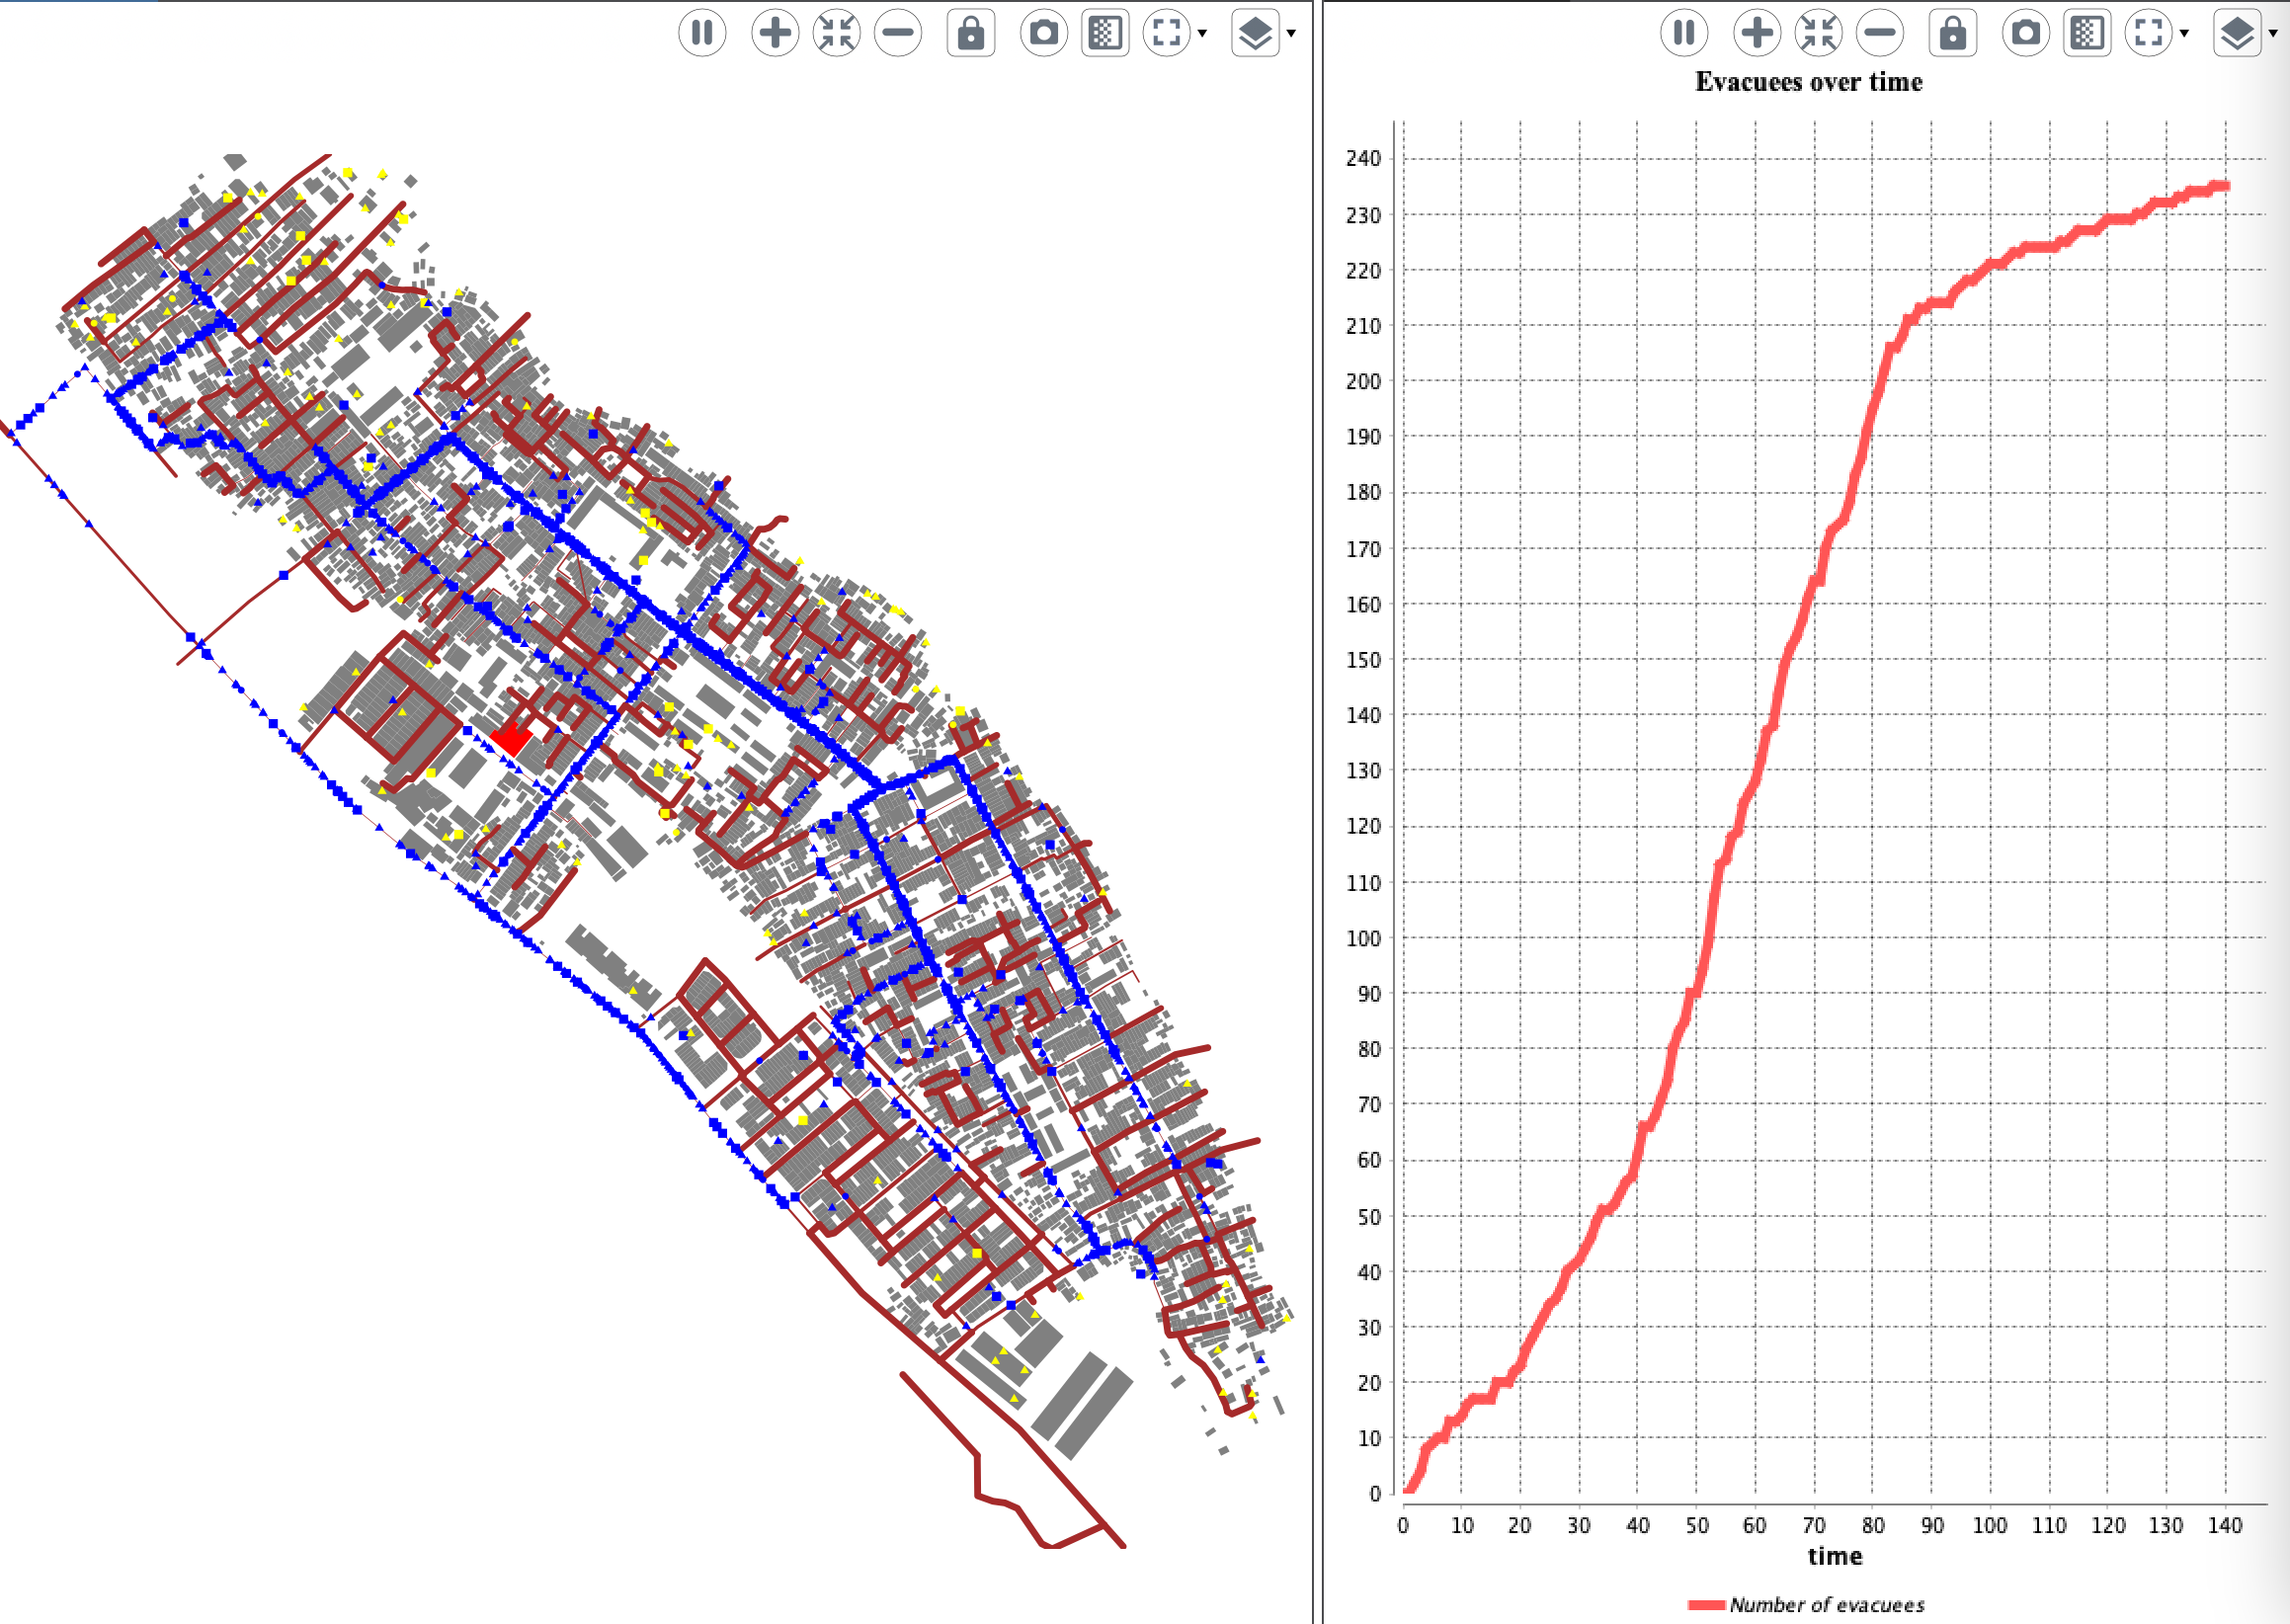
\includegraphics[width=0.8\textwidth]{../images/single-simulation.png}
    \caption{The evacuation simulation with 1000 people, \textbf{random} strategy and 2 hours evacuate time. The right chart is the total number of evacuated people over time. The red building in the right-bottom corner is the shelter.}
    \label{fig:results-single}
\end{figure}

\begin{figure}
    \centering
    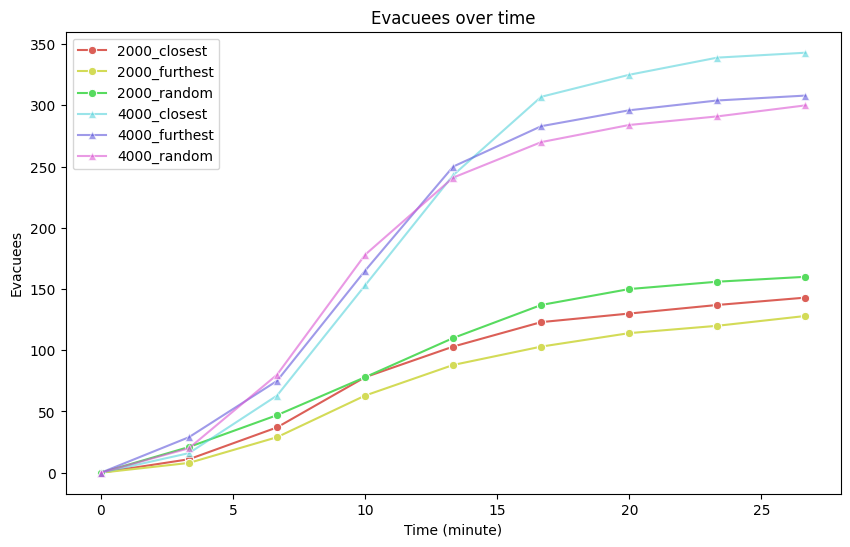
\includegraphics[width=0.8\textwidth]{../images/evacuees_over_time.png}
    \caption{The comparison of the different strategies in number of evacuated people over time.}
    \label{fig:evacuees_over_time}
\end{figure}

Next, I conducted the batch exploration to examine which strategy is the most efficient, which determined in the previous section. The results are presented in the Table \ref{tab:batch}.

\begin{table}[h!]
\centering
\begin{tabular}{|c|c|c|c|c|}
\hline
\textbf{Strategy} & \textbf{No. People} & \textbf{No. Evacuees} & \textbf{Time in roads} & \textbf{Efficiency} \\ \hline
\multirow{4}{*}{random}   & 1500 & 142.4 & 9204840.0  & 0.001858 \\ \cline{2-5} 
                            & 2000 & 180.8 & 12519134.0 & 0.001735 \\ \cline{2-5} 
                            & 3000 & 287.2 & 19016348.0 & 0.001812 \\ \cline{2-5} 
                            & 4000 & \textbf{390.6} & 25555912.0 & 0.001834 \\ \hline
\multirow{4}{*}{furthest} & 1500 & 138.6 & 9116900.0  & 0.001825 \\ \cline{2-5} 
                            & 2000 & 186.4 & 12379352.0 & 0.001811 \\ \cline{2-5} 
                            & 3000 & 291.8 & 18816798.0 & 0.001862 \\ \cline{2-5} 
                            & 4000 & 370.4 & 25506842.0 & 0.001743 \\ \hline
\multirow{4}{*}{closest}  & 1500 & 146.6 & 9048712.0  & \textbf{0.001945} \\ \cline{2-5} 
                            & 2000 & 195.2 & 12304554.0 & 0.001905 \\ \cline{2-5} 
                            & 3000 & 279.2 & 18900030.0 & 0.001773 \\ \cline{2-5} 
                            & 4000 & 371.0 & 25499950.0 & 0.001747 \\ \hline
\end{tabular}
\caption{The results of the batch exploration of the different strategies at alert time of 2 hours.}
\label{tab:batch}
\end{table}

The results show that the \textbf{closest} strategy is the most efficient, followed by the \textbf{furthest} strategy, and the \textbf{random} strategy is the least efficient. The \textbf{closest} strategy is the most efficient because the people closest to the shelter have chance to inform others closed to the shelter as well, which increases the chance of people finding the shelter, and reduce the time wandering in the roads. The \textbf{random} strategy is the strategy that can rescue the largest number of people because the people are randomly selected, which means they are distributed evenly across the map, so the people can start finding the shelter from diverse locations, which reduces the traffic congestion. Compare to the previous experiment of total people evacuated over time, which showed that the \textbf{closest} is the most-saved strategy, but this experiment shows that in the given larger of alert time, the \textbf{random} saves the most people.\\

% --------------------------
% 4. Discussion
% --------------------------
\section{Discussion}

After conducting the simulation, I found that the \textbf{closest} strategy is the most efficient, followed by the \textbf{furthest} strategy, and the \textbf{random} strategy is the least efficient.  The \textbf{random} strategy is the strategy that can rescue the largest number of people because the people are randomly selected, which means they are distributed evenly across the map, so the people can start finding the shelter from diverse locations, which reduces the traffic congestion. \\

With the help of the batch exploration, I can examine the efficiency of the strategies in different settings, which helps to make the comparison between the strategies more reliable. GAMA is very helpful tool in this case, as it allows me to easily implement the agent-based model and conduct the simulation. \\

In the future, I can extend the model by adding more interactions between the inhabitants, with diverse mobilities and behaviors, wide range of information disfusion, and more GIS data to make the simulation more realistic. I can also conduct more experiments with different settings to have a better understanding of the evacuation process and the efficiency of the strategies.\\


% --------------------------
% 4. Discussion
% --------------------------
\section*{Appendix A}

The code is structured in the 3 files:
\begin{itemize}
    \item \textbf{base.gaml}: The base model.
    \item \textbf{simulation.gaml}: The simulation.
    \item \textbf{batch.gaml}: The batch exploration.
\end{itemize}

You can find the code, report and slide, result data in the github link: \url{https://github.com/dungzvu/tsunami-evacuation-simulation}.

\end{document}
